Da es sich bei der Blocklib, mit knapp $60000$ Zeilen Code und über $900$ Java Dateien, um ein großes bereits bestehendes System handelt, ist es unrealistisch, in kurzer Zeit das gesamte Programm so umzustrukturieren, dass es vollständig eine Jobarchitektur nutzt. Diese Umstrukturierung erfordert tiefes Verständnis für jedes zu ändernde System. Zudem müssen viele Bereiche grundlegend geändert werden, um die Abhängigkeiten der Systeme zu verringern beziehungsweise auszuschließen.

Die Blocklib enthält beispielsweise eine Klasse \class{Context}, die als eine Art Singletonimplementierung eines Service Locators~\cite[S.~301~ff.]{Nystrom2015} dient. Da Singletons ähnlich wie globale Variablen von überall aufgerufen werden können, wird der Code dadurch potenziell schwieriger nachvollziehbar~\cite[S.~108]{Nystrom2015}. Dadurch und durch die ebenfalls resultierende Kopplung unterschiedlicher Komponenten würden bei einer naiven Umsetzung der Jobarchitektur unvorhersehbar Wettkampfbedingungen auftreten.
Man erinnere sich, dass Wettkampfbedingungen auftreten wenn nebenläufige Aktivitäten auf die selben Ressourcen zugreifen. Durch den \class{Context} ist es nun schwierig, einen Überblick zu haben von wo aus auf welche Ressourcen zugegriffen wird. Die Wahrscheinlichkeit, dass also Zugriffe existieren, die zu Wettkampfbedingungen führen, ist also sehr hoch, solange dabei nicht sorgsam vorgegangen wird.

\subsection{Design des Renderthreads}
\begin{figure}
	\centering
	\begin{tikzpicture}[scale=1.1]
		\fill[lightgray]  (0,0) rectangle (11,1);
		\fill[lightgray] (0,-1.5) rectangle (11,-0.5);
		\fill[lightgray]  (0,1.5) rectangle (11,2.5);
		
		\node[anchor=east] at (0,2) {Thread 1};
		\node[anchor=east] at (0,0.5) {Thread 2};
		\node[anchor=east] at (0,-1) {Renderthread};
		
		
		\fill [orange,draw=lightgray] (0.5,1.5) rectangle node[black,font=\footnotesize] {Sim 1} (1.5,2.5);
		\fill [orange,draw=lightgray] (0.5,0) rectangle node[black,font=\footnotesize] {Sim 2} (1.5,1);
		\fill [orange,draw=lightgray] (1.5,1.5) rectangle node[black,font=\footnotesize] {Sim 3} (2.5,2.5);
		\fill [orange,draw=lightgray] (2.5,1.5) rectangle node[black,font=\footnotesize] {Sim 4} (3.5,2.5);
		\fill [orange,draw=lightgray] (1.5,0) rectangle node[black,font=\footnotesize] {Sim 5} (2.5,1);
		\fill [orange,draw=lightgray] (3.5,1.5) rectangle node[black,font=\footnotesize] {Sim 6} (4.5,2.5);
		\fill [orange,draw=lightgray] (2.5,0) rectangle node[black,font=\footnotesize] {Sim 7} (3.5,1);
		\fill [orange,draw=lightgray] (3.5,0) rectangle node[black,font=\footnotesize] {Sim 8} (4.5,1);
		
		\fill [orange,draw=lightgray] ($(4.5,0)+(0.5,1.5)$) rectangle node[black,font=\footnotesize] {Sim 1} ($(4.5,0)+(1.5,2.5)$);
		\fill [orange,draw=lightgray] ($(4.5,0)+(0.5,0)$) rectangle node[black,font=\footnotesize] {Sim 2} ($(4.5,0)+(1.5,1)$);
		\fill [orange,draw=lightgray] ($(4.5,0)+(1.5,1.5)$) rectangle node[black,font=\footnotesize] {Sim 3} ($(4.5,0)+(2.5,2.5)$);
		\fill [orange,draw=lightgray] ($(4.5,0)+(2.5,1.5)$) rectangle node[black,font=\footnotesize] {Sim 5} ($(4.5,0)+(3.5,2.5)$);
		\fill [orange,draw=lightgray] ($(4.5,0)+(1.5,0)$) rectangle node[black,font=\footnotesize] {Sim 4} ($(4.5,0)+(2.5,1)$);
		\fill [orange,draw=lightgray] ($(4.5,0)+(3.5,1.5)$) rectangle node[black,font=\footnotesize] {Sim 6} ($(4.5,0)+(4.5,2.5)$);
		\fill [orange,draw=lightgray] ($(4.5,0)+(2.5,0)$) rectangle node[black,font=\footnotesize] {Sim 7} ($(4.5,0)+(3.5,1)$);
		\fill [orange,draw=lightgray] ($(4.5,0)+(3.5,0)$) rectangle node[black,font=\footnotesize] {Sim 8} ($(4.5,0)+(4.5,1)$);
	
		\fill [magenta] (0.5,-0.5) rectangle node[black]{Render $n-1$} (4.2,-1.5);
		\fill [magenta] (5,-0.5) rectangle node[black]{Render $n$} (8.7,-1.5);
		
		\node at (2.5,3.5) {Frame $n$};
		\node at (7,3.5) {Frame $n+1$};
		
		\draw  (0.5,3) rectangle (4.5,-2);
		\draw  (5,3) rectangle (9,-2);
	\end{tikzpicture}
	\caption{Darstellung des Designs der Multithreading Architektur der Blocklib. Es existiert ein gesonderter Renderthread, der einen großen Teil der Rechenzeit während eines Frames nutzt.}\label{fig:optimalArchitecture}
	\todo{Caption}
\end{figure}

Da der Performancegewinn, in Form von \ac{fps}, bei der Nutzung eines Renderthreads als hoch zu erwarten ist, soll dieser in die Blocklib integriert werden. Um die Anforderungen von Kapitel~\ref{sec:anforderungen} zu Erfüllen, wird ein Jobsystem implementiert. Da die Blocklib OpenGL als Grafik Schnittstelle nutzt und OpenGL, wie in Abschnitt~\ref{sec:gamesJobsystem} beschrieben, Multithreading nicht unterstützt, kann das Rendering selbst nicht nebenläufig durchgeführt werden.

Der Renderthread kann einerseits als Teil des Jobsystems designt werden, andererseits gibt es die Möglichkeit den Renderthread von diesem zu trennen. Ist der Renderthread Teil des Jobsystems, kann dieser voll zur Bearbeitung von Jobs mitgenutzt werden. Da üblicherweise die Anzahl der Threads der Anzahl der Prozessorkerne entspricht, kann man so automatisch immer die Leistung aller Prozessorkerne nutzen. Trennt man den Thread dagegen ab, entsteht die Problematik zu entscheiden, wann welche Anzahl von Threads genutzt wird, um möglichst alle Kerne zu nutzen, aber gleichzeitig zu verhindern, dass sich die Threads in der Ausführung gegenseitig behindern. Andererseits gestaltet sich die Implementierung eines getrennten Renderthreads als deutlich einfacher und intuitiver~\cite{Tatarchuk2014}, im Gegensatz zur Jobsystemintegration.

Nach Messungen ergibt sich, dass das Rendering in etwa \SI{50}{\percent}\todo{messen} der Zeit eines Frames benötigt. Daher bietet es sich an, den Renderthread zu separieren. Der prinzipiell mögliche Performancegewinn durch die Integration in das Jobsystem ist ausgeschlossen, da das Rendering selbst sie gesamte Rechenleistung des Kerns jeden Frame beansprucht. Da das Rendering im sequentialisierten Fall circa \SI{50}{\percent} der Zeit benötigt, entspricht das annähernd \SI{100}{\percent}, sobald Simulation und Rendering in zwei Threads nebenläufig ausgeführt werden. Wird die Simulation selbst nebenläufig durchgeführt verstärkt sich dieser Effekt, wodurch die Framezeit, durch das Rendering bestimmt wird. Damit lässt sich auch die Anzahl der Threads des Jobsystems bestimmen, indem die Anzahl der Jobthreads um eins verringert wird ohne dadurch Prozessorkerne ohne Arbeit zu verursachen.

Da der Renderthread auf Daten des Spiels zugreift, um die sichtbaren Elemente zu zeichnen, muss sichergestellt werden, dass diese Daten keinen Wettkampfbedingungen unterliegen. In der Spieleentwicklung ist es üblich einen \emph{Spielzustand} (engl. Game State) zu definieren, der während der Simulation in jedem Frame angepasst wird. Der Teil des Zustandes auf den der Renderthread zugreift muss also konstant sein. Während der Simulation wird dieser allerdigs verändert. Eine Möglichkeit, dieses Problem zu beheben, besteht darin einen \emph{Double Buffer}~\cite[S.~143]{Nystrom2015} zu nutzen, um den gesamten Spielzustand zwischenzuspeichern~\cite{Tatarchuk2014}. Die Blocklib ist nicht mit diesem Hintergrund entwickelt worden, weswegen es keine einfache Möglichkeit gibt, den gesamten Spielzustand auf diese Weise zwischenzuspeichern. Die Objekte, die den Spielzustand darstellen, sind über die Blocklib hinweg verteilt. Um dennoch einen Renderthread nutzen zu können, müssen die Objekte identifiziert werden, die für das Rendering benötigt werden. Für diese Objekte muss dann ein geeigneter Double Buffer erzeugt werden, sodass die Daten aus Renderthread-Sicht konstant sind.

Somit ist eine nebenläufige Architektur, wie sie in Abbildung~\ref{fig:optimalArchitecture} dargestellt wird, erstrebenswert. Es gibt einen Renderthread, der die von der Simulation im vorherigen Frame berechneten Objekte zeichnet. Alle anderen verfügbaren Hardwarethreads können in dem Jobsystem für die Simulation genutzt werden. 

\subsection{Design des Jobsystems}
\begin{figure}
	\centering
	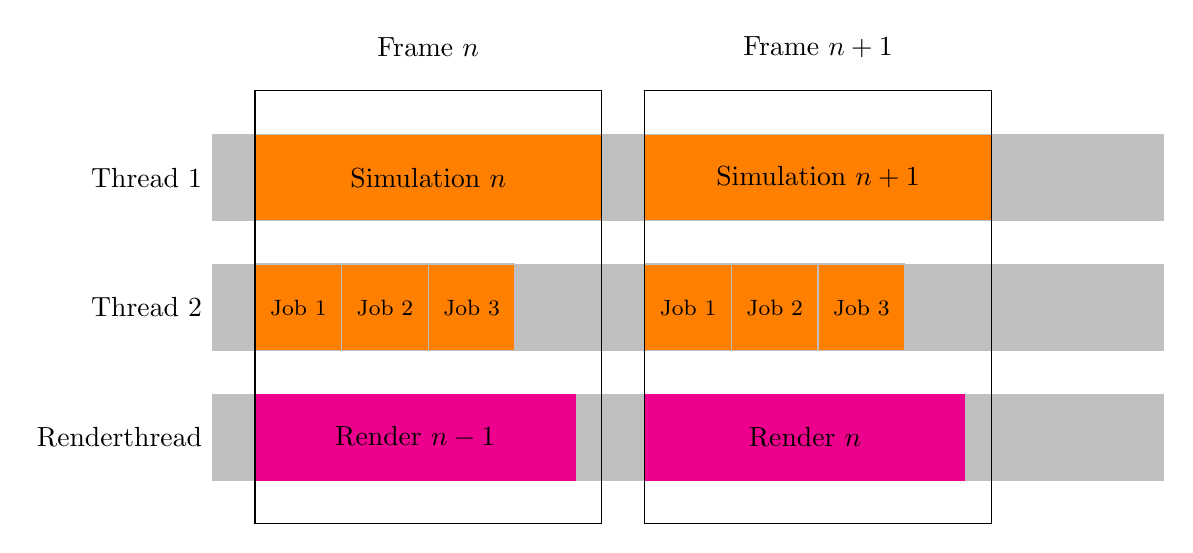
\begin{tikzpicture}[scale=1.1]
		\fill[lightgray]  (0,0) rectangle (11,1);
		\fill[lightgray] (0,-1.5) rectangle (11,-0.5);
		\fill[lightgray]  (0,1.5) rectangle (11,2.5);
		
		\node[anchor=east] at (0,2) {Thread 1};
		\node[anchor=east] at (0,0.5) {Thread 2};
		\node[anchor=east] at (0,-1) {Renderthread};
		
		
		\fill [orange,draw=lightgray] (0.5,1.5) rectangle node[black] {Simulation $n$} (4.5,2.5);
		\fill [orange,draw=lightgray] (0.5,0) rectangle node[black,font=\footnotesize] {Job 1} (1.5,1);
		\fill [orange,draw=lightgray] (1.5,0) rectangle node[black,font=\footnotesize] {Job 2} (2.5,1);
		\fill [orange,draw=lightgray] (2.5,0) rectangle node[black,font=\footnotesize] {Job 3} (3.5,1);
	
		\fill [orange,draw=lightgray] (5,1.5) rectangle node[black] {Simulation $n+1$} (9,2.5);
		\fill [orange,draw=lightgray] (5,0) rectangle node[black,font=\footnotesize] {Job 1} (6,1);
		\fill [orange,draw=lightgray] (6,0) rectangle node[black,font=\footnotesize] {Job 2} (7,1);
		\fill [orange,draw=lightgray] (7,0) rectangle node[black,font=\footnotesize] {Job 3} (8,1);
	
		\fill [magenta] (0.5,-0.5) rectangle node[black]{Render $n-1$} (4.2,-1.5);
		\fill [magenta] (5,-0.5) rectangle node[black]{Render $n$} (8.7,-1.5);
		
		\node at (2.5,3.5) {Frame $n$};
		\node at (7,3.5) {Frame $n+1$};
		
		\draw  (0.5,3) rectangle (4.5,-2);
		\draw  (5,3) rectangle (9,-2);
	\end{tikzpicture}
	\caption{Design der Threadingarchitektur der Blocklib}\label{fig:plannedArchitecture}
	\todo{Caption}
\end{figure}

Aufgrund des Umfangs der Blocklib und der Unübersichtlichkeit an einigen Stellen kann das Jobsystem nicht, wie in Abbildung~\ref{fig:optimalArchitecture} gezeigt, umfassend integriert werden. Um die Anforderungen von Kapitel~\ref{sec:anforderungen} zu erfüllen, wird daher ein Jobsystem implementiert, das nur an ausgewählten Stellen mit der Blocklib konsolidiert wird und ansonsten für die zukünftige Nutzung bereitsteht.

Da das Jobsystem keine vollständige Integration in die Blocklib erfährt, verändert sich die Architektur konzeptuell leicht. Diese Änderung ist in Abbildung~\ref{fig:plannedArchitecture} zu sehen. Anstatt die gesamte Simulation in viele kleine Jobs zu zerlegen, gibt es eine sequentialisierte Simulation, die dann aber die Möglichkeit besitzt, weitere Jobs zu starten. Mit dieser Architektur ist es allerdings möglich, die Blocklib inkrementell zu der in Abbildung~\ref{fig:optimalArchitecture} gezeigten Architektur umzuwandeln, indem immer mehr pseudosequentialisierte Anweisungen in als nebenläufige Jobs definiert werden. 